\chapter{Conditionals and logic}

\index{boolean}
\index{type!boolean}

The programs we've seen in previous chapters do pretty much the same thing every time, regardless of the input.
For more complex computations, programs usually react to the inputs, check for certain conditions, and generate appropriate results.
This chapter presents the features you need for programs to make decisions: a new data type called \java{boolean}, operators for expressing logic, and \java{if} statements.

%\java{boolean} is named after George Boole, who developed a formal system that represents logic using the values {\em true} and {\em false} and operations like {\em and}, {\em or}, and {\em not}.
%In Java, the values \java{true} and \java{false} belong to the data type \java{boolean}.

%\java{true} and \java{false} are special values in Java, and together they make up a type called {\bf boolean}.
%You might recall that when I defined a type, I said it was a set of values.
%In the case of \java{int}s, \java{double}s and \java{String}s, those sets are pretty big.
%For \java{boolean}s, there are only two values.
%The values \java{true} and \java{false} are keywords in Java, so they may appear in a different color, depending on your development environment.


\section{Relational operators}

\index{operator!relational}
\index{relational operator}
\index{comparison operator}

{\bf Relational operators} are used to check conditions like whether two values are equal, or whether one is greater than the other.
The following expressions show how they are used:

\begin{code}
x == y          // x is equal to y
x != y          // x is not equal to y
x > y           // x is greater than y
x < y           // x is less than y
x >= y          // x is greater than or equal to y
x <= y          // x is less than or equal to y
\end{code}

The result of a relational operator is one of two special values, \java{true} or \java{false}.
These values belong to the data type \java{boolean}; in fact, they are the only boolean values.

\index{assignment}
\index{operator!assignment}

You are probably familiar with these operations, but notice that the Java operators are different from the mathematical symbols like $=$, $\neq$, and $\le$.
A common error is to use a single \java{=} instead of a double \java{==}.
Remember that \java{=} is the assignment operator, and \java{==} is a comparison operator.
Also, there is no such thing as the \java{=<} or \java{=>} operators.

The two sides of a relational operator have to be compatible.
For example, the expression \java{5 < "6"} is invalid because \java{5} is an \java{int} and \java{"6"} is a \java{String}.
When comparing values of different numeric types, Java applies the same conversion rules we saw previously with the assignment operator.
For example, when evaluating the expression \java{5 < 6.0}, Java automatically converts the \java{5} to \java{5.0}.

Most relational operators don't work with strings.
But confusingly, \java{==} and \java{!=} do work with strings -- they just don't do what you expect.
We'll explain what they do later; in the meantime, don't use them with strings.
Instead, you should use the \java{equals} method:

\begin{code}
String fruit1 = "Apple";
String fruit2 = "Orange";
System.out.println(fruit1.equals(fruit2));
\end{code}

The result of \java{fruit1.equals(fruit2)} is the boolean value \java{false}.


\section{Logical operators}

\index{logical operator}
\index{operator!logical}

Java has three {\bf logical operators}: \java{&&}, \java{||}, and \java{!}, which respectively stand for {\em and}, {\em or}, and {\em not}.
The results of these operators are similar to their meanings in English.

For example, \java{x > 0 && x < 10} is true when \java{x} is both greater than zero {\em and} less than 10.
The expression \java{evenFlag || n \% 3 == 0} is true if either condition is true, that is, if \java{evenFlag} is true {\em or} the number \java{n} is divisible by 3.
Finally, the \java{!} operator inverts a boolean expression.
So \java{!evenFlag} is true if \java{evenFlag} is {\em not} true.

\index{short circuit}

Logical operators evaluate the second expression only when necessary.
For example, \java{true || anything} is always true, so Java does not need to evaluate the expression \java{anything}.
Likewise, \java{false && anything} is always false.
Ignoring the second operand, when possible, is called {\bf short circuit} evaluation, by analogy with an electrical circuit.
Short circuit evaluation can save time, especially if \java{anything} takes a long time to evaluate.
It can also avoid unnecessary errors, if \java{anything} might fail.

\index{De Morgan's laws}

If you ever have to negate an expression that contains logical operators, and you probably will, {\bf De Morgan's laws} can help:

\begin{itemize}
\item \java{!(A && B)} ~is the same as~ \java{!A || !B}
\item \java{!(A || B)} ~is the same as~ \java{!A && !B}
\end{itemize}

Negating a logical expression is the same as negating each term and changing the operator.
The \java{!} operator takes precedence over \java{&&} and \java{||}, so you don't have to put parentheses around the individual terms \java{!A} and \java{!B}.

De Morgan's laws also apply to the relational operators.
In this case, negating each term means using the ``opposite'' relational operator.

\begin{itemize}
\item \java{!(x < 5 && y == 3)} ~is the same as~ \java{x >= 5 || y != 3}
\item \java{!(x >= 1 || y != 7)} ~is the same as~ \java{x < 1 && y == 7}
\end{itemize}

It may help to read these examples out loud in English.
For instance, ``If I don't want the case where $x$ is less than 5 and $y$ is 3, then I need $x$ to be greater than or equal to 5, or I need $y$ to be anything but 3.''


\section{Conditional statements}

\index{conditional statement}
\index{statement!conditional}
\index{if statement}
\index{statement!if}

To write useful programs, we almost always need to check conditions and react accordingly.
{\bf Conditional statements} give us this ability.
The simplest conditional statement in Java is the \java{if} statement:

\begin{code}
if (x > 0) {
    System.out.println("x is positive");
}
\end{code}

The expression in parentheses is called the condition.
If it is true, the statements in braces get executed.
If the condition is false, execution skips over that block of code.
The condition in parentheses can be any boolean expression.

\index{branch}
\index{statement!else}

A second form of conditional statement has two possibilities, indicated by \java{if} and \java{else}.
The possibilities are called {\bf branches}, and the condition determines which one gets executed:

\begin{code}
if (x % 2 == 0) {
    System.out.println("x is even");
} else {
    System.out.println("x is odd");
}
\end{code}

If the remainder when \java{x} is divided by 2 is zero, we know that \java{x} is even, and this fragment displays a message to that effect.
If the condition is false, the second print statement is executed instead.
Since the condition must be true or false, exactly one of the branches will run.

The braces are optional for branches that have only one statement.
So we could have written the previous example this way:

\begin{code}
if (x % 2 == 0)
    System.out.println("x is even");
else
    System.out.println("x is odd");
\end{code}

However, it's better to use braces -- even when they are optional -- to avoid making the mistake of adding statements to an \java{if} or \java{else} block and forgetting to add the braces.

\begin{code}
if (x > 0)
    System.out.println("x is positive");
    System.out.println("x is not zero");
\end{code}

This code is misleading because it's not indented correctly.
Since there are no braces, only the first \java{println} is part of the \java{if} statement.
Here is what the compiler actually sees:

\begin{code}
if (x > 0) {
    System.out.println("x is positive");
}
    System.out.println("x is not zero");
\end{code}

As a result, the second \java{println} runs no matter what.
Even experienced programmers make this mistake; search the web for Apple's ``goto fail'' bug.


\section{Chaining and nesting}

\index{chaining}

Sometimes you want to check related conditions and choose one of several actions.
One way to do this is by {\bf chaining} a series of \java{if} and \java{else} statements:

\begin{code}
if (x > 0) {
    System.out.println("x is positive");
} else if (x < 0) {
    System.out.println("x is negative");
} else {
    System.out.println("x is zero");
}
\end{code}

These chains can be as long as you want, although they can be difficult to read if they get out of hand.
One way to make them easier to read is to use standard indentation, as demonstrated in these examples.
If you keep all the statements and braces lined up, you are less likely to make syntax errors.

\index{nesting}

In addition to chaining, you can also make complex decisions by {\bf nesting} one conditional statement inside another.
We could have written the previous example as:

\begin{code}
if (x == 0) {
    System.out.println("x is zero");
} else {
    if (x > 0) {
        System.out.println("x is positive");
    } else {
        System.out.println("x is negative");
    }
}
\end{code}

The outer conditional has two branches.
The first branch contains a \java{print} statement, and the second branch contains another conditional statement, which has two branches of its own.
These two branches are also \java{print} statements, but they could have been conditional statements as well.

These kinds of nested structures are common, but they get difficult to read very quickly.
Good indentation is essential to make the structure (or intended structure) apparent to the reader.


\section{Flag variables}

\index{expression!boolean}

To store a \java{true} or \java{false} value, you need a \java{boolean} variable.
You can create one like this:

\begin{code}
boolean flag;
flag = true;
boolean testResult = false;
\end{code}

\index{initialize}
\index{statement!initialization}

The first line is a variable declaration, the second is an assignment, and the third is both.
Since relational operators evaluate to a \java{boolean} value, you can store the result of a comparison in a variable:

\begin{code}
boolean evenFlag = (n % 2 == 0);    // true if n is even
boolean positiveFlag = (x > 0);     // true if x is positive
\end{code}

\index{flag}

The parentheses are unnecessary, but they make the code easier to read.
A variable defined in this way is called a {\bf flag}, because it signals or ``flags'' the presence or absence of a condition.

You can use flag variables as part of a conditional statement later:

\begin{code}
if (evenFlag) {
    System.out.println("n was even when I checked it");
}
\end{code}

Notice that you don't have to write \java{if (evenFlag == true)}.
Since \java{evenFlag} is a \java{boolean}, it's already a condition.
Likewise, to check if a flag is \java{false}:

\begin{code}
if (!evenFlag) {
    System.out.println("n was odd when I checked it");
}
\end{code}


\section{The return statement}

\index{return}
\index{statement!return}

The \java{return} statement allows you to terminate a method before you reach the end of it.
One reason to use \java{return} is if you detect an error condition:

\begin{code}
public static void printLogarithm(double x) {
    if (x <= 0.0) {
        System.err.println("Error: x must be positive.");
        return;
    }
    double result = Math.log(x);
    System.out.println("The log of x is " + result);
}
\end{code}

\index{logarithm}

This example defines a method named \java{printLogarithm} that takes a \java{double} value (named \java{x}) as a parameter.
It checks whether \java{x} is less than or equal to zero, in which case it displays an error message and then uses \java{return} to exit the method.
The flow of execution immediately returns to where the method was invoked, and the remaining lines of the method are not executed.

\index{System.err}

This example uses \java{System.err}, which is an \java{OutputStream} normally used for error messages and warnings.
Some development environments display output to \java{System.err} with a different color or in a separate window.


\section{Validating input}
\label{validate}

Here is a method that uses \java{printLogarithm} from the previous section:

\begin{code}
public static void scanDouble(Scanner in) {
    System.out.print("Enter a number: ");
    double x = in.nextDouble();
    printLogarithm(x);
}
\end{code}

This example uses \java{nextDouble}, so the \java{Scanner} (provided by the \java{main} method) tries to read a \java{double}.
If the user enters a floating-point number, the \java{Scanner} converts it to a \java{double}.
But if the user types anything else, the \java{Scanner} throws an \java{InputMismatchException}.

\index{exception!InputMismatch}
\index{InputMismatchException}

We can prevent this error by checking the input before parsing it:

\begin{code}
public static void scanDouble(Scanner in) {
    System.out.print("Enter a number: ");
    if (!in.hasNextDouble()) {
        String word = in.next();
        System.err.println(word + " is not a number");
        return;
    }
    double x = in.nextDouble();
    printLogarithm(x);
}
\end{code}

The \java{Scanner} class provides \java{hasNextDouble}, which checks whether the next token in the input stream can be interpreted as a \java{double}.
If so, we can call \java{nextDouble} with no chance of throwing an exception.
If not, we display an error message and return.
%Returning from \java{main} terminates the program.

%Notice the use of the \java{!} operator, instead of the test \java{in.hasNextDouble() == false}.
%Since the \java{hasNextDouble} method returns a boolean result, it is already a condition.


\section{Recursive methods}
\label{recursion}

\index{recursion}

Now that we have conditional statements, we can explore one of the most magical things a program can do: {\bf recursion}.
Consider the following example:

\begin{code}
public static void countdown(int n) {
    if (n == 0) {
        System.out.println("Blastoff!");
    } else {
        System.out.println(n);
        countdown(n - 1);
    }
}
\end{code}

\index{recursive}

The name of the method is \java{countdown}; it takes a single integer as a parameter.
If the parameter is zero, it displays the word ``Blastoff''.
Otherwise, it displays the number and then invokes {\em itself}, passing \java{n - 1} as the argument.
A method that invokes itself is called {\bf recursive}.

What happens if we invoke \java{countdown(3)} from \java{main}?

\vspace{-1ex}
\begin{quote}
The execution of \java{countdown} begins with \java{n == 3}, and since \java{n} is not zero, it displays the value 3, and then invokes itself...
\begin{quote}
The execution of \java{countdown} begins with \java{n == 2}, and since \java{n} is not zero, it displays the value 2, and then invokes itself...
\begin{quote}
The execution of \java{countdown} begins with \java{n == 1}, and since \java{n} is not zero, it displays the value 1, and then invokes itself...
\begin{quote}
The execution of \java{countdown} begins with \java{n == 0}, and since \java{n} is zero, it displays the word ``Blastoff!'' and then returns.
\end{quote}
The \java{countdown} that got \java{n == 1} returns.
\end{quote}
The \java{countdown} that got \java{n == 2} returns.
\end{quote}
The \java{countdown} that got \java{n == 3} returns.
\end{quote}
\vspace{-1ex}

And then you're back in \java{main}.
So the total output looks like:

\begin{stdout}
3
2
1
Blastoff!
\end{stdout}

As a second example, we'll rewrite the methods \java{newLine} and \java{threeLine} from Section~\ref{adding_methods}.

\begin{code}
public static void newLine() {
    System.out.println();
}

public static void threeLine() {
    newLine();
    newLine();
    newLine();
}
\end{code}

\index{newline}

Although these methods work, they would not help if we wanted to display two newlines, or maybe 100.
A better alternative would be:

\begin{code}
public static void nLines(int n) {
    if (n > 0) {
        System.out.println();
        nLines(n - 1);
    }
}
\end{code}

This method takes an integer, \java{n}, as a parameter and displays \java{n} newlines.
The structure is similar to \java{countdown}.
As long as $n$ is greater than zero, it displays a newline and then invokes itself to display $(n-1)$ additional newlines.
The total number of newlines is $1 + (n - 1)$, which is just what we wanted: $n$.


\section{Recursive stack diagrams}

\index{stack diagram}
\index{diagram!stack}

In the previous chapter, we used a stack diagram to represent the state of a program during a method invocation.
The same kind of diagram can make it easier to interpret a recursive method.

Remember that every time a method gets called, Java creates a new frame that contains the current method's parameters and variables.
Figure~\ref{fig.stack2} is a stack diagram for \java{countdown}, called with \java{n == 3}.

\begin{figure}[!ht]
\begin{center}
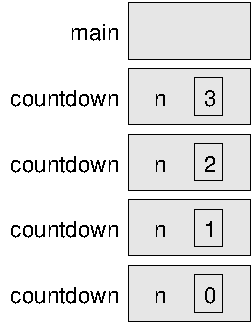
\includegraphics{figs/stack2.pdf}
\caption{Stack diagram for the \java{countdown} program.}
\label{fig.stack2}
\end{center}
\end{figure}

By convention, the stack for \java{main} is at the top and the stack grows down.
The frame for \java{main} is empty because \java{main} does not have any variables.
(It has the parameter \java{args}, but since we're not using it, we left it out of the diagram.)

\index{base case}

There are four frames for \java{countdown}, each with a different value for the parameter \java{n}.
The last frame, with \java{n == 0}, is called the {\bf base case}.
It does not make a recursive call, so there are no more frames below it.

If there is no base case in a recursive method, or if the base case is never reached, the stack would grow forever, at least in theory.
In practice, the size of the stack is limited; if you exceed the limit, you get a \java{StackOverflowError}.

For example, here is a recursive method without a base case:

\begin{code}
public static void forever(String s) {
    System.out.println(s);
    forever(s);
}
\end{code}

\index{call stack}
\index{stack overflow}

This method displays the string until the stack overflows, at which point it throws an exception.


\section{Binary numbers}

The \java{countdown} example has three parts: (1) it checks the base case, (2) displays something, and (3) makes a recursive call.
What do you think happens if you reverse steps 2 and 3, making the recursive call {\em before} displaying?

\begin{code}
public static void countup(int n) {
    if (n == 0) {
        System.out.println("Blastoff!");
    } else {
        countup(n - 1);
        System.out.println(n);
    }
}
\end{code}

The stack diagram is the same as before, and the method is still called $n$ times.
But now the \java{System.out.println} happens just before each recursive call returns.
As a result, it counts up instead of down:

\begin{stdout}
Blastoff!
1
2
3
\end{stdout}

\index{binary}

This behavior comes in handy when it is easier to compute results in reverse order.
For example, to convert a decimal integer into its {\bf binary} representation, you repeatedly divide the number by two:

\begin{stdout}
23 / 2 is 11 remainder 1
11 / 2 is  5 remainder 1
 5 / 2 is  2 remainder 1
 2 / 2 is  1 remainder 0
 1 / 2 is  0 remainder 1
\end{stdout}

Reading these remainders from bottom to top, 23 in binary is 10111.
For more background about binary numbers, see \url{http://www.mathsisfun.com/binary-number-system.html}.

Here is a recursive method that displays the binary representation of any positive integer:

\begin{code}
public static void displayBinary(int value) {
    if (value > 0) {
        displayBinary(value / 2);
        System.out.print(value % 2);
    }
}
\end{code}

If \java{value} is zero, \java{displayBinary} does nothing (that's the base case).
If the argument is positive, the method divides it by two and calls \java{displayBinary} recursively.
When the recursive call returns, the method displays one digit of the result and returns (again).

The leftmost digit is at the bottom of the stack, so it gets displayed first.
The rightmost digit, at the top of the stack, gets displayed last.
After invoking \java{displayBinary}, we use \java{println} to complete the output.

\begin{code}
displayBinary(23);
System.out.println();
// output is 10111
\end{code}

Learning to think recursively is an important aspect of learning to think like a computer scientist.
Many algorithms can be written concisely with recursive methods that perform computations on the way down, on the way up, or both.


\section{Vocabulary}

\begin{description}

\term{boolean}
A data type with only two values, \java{true} and \java{false}.

\index{operator!relational}
\term{relational operator}
An operator that compares two values and produces a \java{boolean} indicating the relationship between them.

\index{operator!logical}
\term{logical operator}
An operator that combines boolean values and produces a boolean value.

\term{short circuit}
A way of evaluating logical operators that only evaluates the second operand if necessary.

\term{De Morgan's laws}
Mathematical rules that show how to negate a logical expression.

\term{conditional statement}
A statement that uses a condition to determine which statements to execute.

\term{branch}
One of the alternative sets of statements inside a conditional statement.

\term{chaining}
A way of joining several conditional statements in sequence.

\term{nesting}
Putting a conditional statement inside one or both branches of another conditional statement.

\term{flag}
A variable (usually \java{boolean}) that represents a condition or status.

\term{recursion}
The process of invoking (and restarting) the same method that is currently executing.

\term{recursive}
A method that invokes itself, usually with different arguments.

\term{base case}
A condition that causes a recursive method {\em not} to make another recursive call.

\term{binary}
A system that uses only zeros and ones to represent numbers.
Also known as ``base 2''.

\end{description}


\section{Exercises}

The code for this chapter is in the {\tt ch05} directory of {\tt ThinkJavaCode}.
See page~\pageref{code} for instructions on how to download the repository.
Before you start the exercises, we recommend that you compile and run the examples.

If you have not already read Appendix~\ref{debugger}, now might be a good time.
It describes the DrJava debugger, which is a useful tool for tracing the flow of execution.


\begin{exercise}

Logical operators can simplify nested conditional statements.
For example, can you rewrite this code using a single \java{if} statement?

\begin{code}
if (x > 0) {
    if (x < 10) {
        System.out.println("positive single digit number.");
    }
}
\end{code}

\end{exercise}


\begin{exercise}
For the following program:

\begin{enumerate}

\item Draw a stack diagram that shows the state of the program the {\it second} time \java{zoop} is invoked.

\item What is the complete output?

\end{enumerate}

\begin{code}
public static void zoop(String fred, int bob) {
    System.out.println(fred);
    if (bob == 5) {
        ping("not ");
    } else {
        System.out.println("!");
    }
}

public static void main(String[] args) {
    int bizz = 5;
    int buzz = 2;
    zoop("just for", bizz);
    clink(2 * buzz);
}
\end{code}

\begin{code}
public static void clink(int fork) {
    System.out.print("It's ");
    zoop("breakfast ", fork);
}

public static void ping(String strangStrung) {
    System.out.println("any " + strangStrung + "more ");
}
\end{code}
\end{exercise}


\begin{exercise}

Draw a stack diagram that shows the state of the program in Section~\ref{recursion} after \java{main} invokes \java{nLines} with the parameter \java{n == 4}, just before the last invocation of \java{nLines} returns.

\end{exercise}


\begin{exercise}

Fermat's Last Theorem says that there are no integers $a$, $b$, and $c$ such that $a^n + b^n = c^n$, except when $n \leq 2$.

Write a method named \java{checkFermat} that takes four integers as parameters -- \java{a}, \java{b}, \java{c} and \java{n} -- and checks to see if Fermat's theorem holds.
If $n$ is greater than 2 and $a^n + b^n = c^n$, the program should display ``Holy smokes, Fermat was wrong!''
Otherwise the program should display ``No, that doesn't work.''

{\it Hint:} You may want to use \java{Math.pow}.

\end{exercise}


\begin{exercise}

The purpose of this exercise is to take a problem and break it into smaller problems, and to solve the smaller problems by writing simple methods.
Consider the first verse of the song ``99 Bottles of Beer'':

\begin{quote}
99 bottles of beer on the wall,\\
99 bottles of beer,\\
ya' take one down, ya' pass it around,\\
98 bottles of beer on the wall.
\end{quote}

Subsequent verses are identical except that the number of bottles gets smaller by one in each verse, until the last verse:

\begin{quote}
No bottles of beer on the wall,\\
no bottles of beer,\\
ya' can't take one down, ya' can't pass it around,\\
'cause there are no more bottles of beer on the wall!
\end{quote}

And then the song (finally) ends.

Write a program that displays the entire lyrics of ``99 Bottles of Beer''.
Your program should include a recursive method that does the hard part, but you might want to write additional methods to separate other parts of the program.
As you develop your code, test it with a small number of verses, like \java{3}.

\end{exercise}


\begin{exercise}

This exercise reviews the flow of execution through a program with multiple methods.
Read the following code and answer the questions.

\begin{code}
public class Buzz {

    public static void baffle(String blimp) {
        System.out.println(blimp);
        zippo("ping", -5);
    }

    public static void zippo(String quince, int flag) {
        if (flag < 0) {
            System.out.println(quince + " zoop");
        } else {
            System.out.println("ik");
            baffle(quince);
            System.out.println("boo-wa-ha-ha");
        }
    }

    public static void main(String[] args) {
        zippo("rattle", 13);
    }

}
\end{code}

\begin{enumerate}

\item Write the number {\tt 1} next to the first line of code in this program that will execute.

\item Write the number {\tt 2} next to the second line of code, and so on until the end of the program.
If a line is executed more than once, it might end up with more than one number next to it.

\item What is the value of the parameter \java{blimp} when \java{baffle} gets invoked?

\item What is the output of this program?

\end{enumerate}

\end{exercise}


\begin{exercise}

Now that we have conditional statements, we can get back to the ``Guess My Number'' game from Exercise~\ref{guess}.

You should already have a program that chooses a random number, prompts the user to guess it, and displays the difference between the guess and the chosen number.

Adding a small amount of code at a time, and testing as you go, modify the program so it tells the user whether the guess is too high or too low, and then prompts the user for another guess.

The program should continue until the user gets it right.
{\it Hint:} Use two methods, and make one of them recursive.

\end{exercise}
